\documentclass{article}

% 导入宏包
\usepackage{fancyhdr}
\usepackage{ctex}
\usepackage{listings}
\usepackage{graphicx}
\usepackage[a4paper, body={18cm,22cm}]{geometry}
\usepackage{amsmath,amsthm,amssymb,amstext,wasysym,enumerate,graphicx}
\usepackage{float,abstract,booktabs,indentfirst,amsmath}
\usepackage{array}
\usepackage{multirow}
\usepackage{url}
\usepackage{diagbox}
\usepackage{enumitem}
\usepackage{xcolor}
\usepackage{makecell}
\usepackage{tcolorbox}
\usepackage{tikz}
\usetikzlibrary{shapes,arrows.meta,positioning}
\usepackage[bookmarks=true, colorlinks, citecolor=blue, linkcolor=black]{hyperref}


% 设置段落
\renewcommand\arraystretch{1.4}
\setlength{\parindent}{2em}
\setCJKmonofont{黑体}

% 设置高亮文字
\newtcbox{\mybox}[1][red]
{on line, arc = 0pt, outer arc = 0pt,
	colback = #1!10!white, colframe = #1!50!black,
	boxsep = 0pt, left = 1pt, right = 1pt, top = 2pt, bottom = 2pt,
	boxrule = 0pt, bottomrule = 1pt, toprule = 1pt}

% 配置代码显示
\lstset{
	xleftmargin = 3em,
	xrightmargin = 3em,
	aboveskip = 1em,
	backgroundcolor = \color{white},
	basicstyle = \small\ttfamily,
	rulesepcolor = \color{gray},
	breaklines = true,
	numbers = left,
	numberstyle = \small,
	numbersep = -14pt,
	keywordstyle = \color{purple}\bfseries,
	commentstyle = \color{green!60!black}, % 修改注释颜色
	stringstyle = \color{red!60!green!90!blue!90},
	morekeywords = {ASSERT, int64_t, uint32_t},
	moreemph = {ASSERT, NULL},
	emphstyle = \color{red}\bfseries,
	moreemph = [2]{int64\_t, uint32\_t, tid\_t, uint8\_t, int16\_t, uint16\_t, int32\_t, size\_t, bool},
	emphstyle = [2]\color{purple}\bfseries,
	frame = shadowbox,
	showspaces = false,
	columns = fixed
	morecomment = [l][\color{green!60!black}]{+}, % 设置以+开头的代码行为绿色
}

%--------------------页眉--------------------%

\pagestyle{fancy}
\fancyhead[L]{}
\fancyhead[R]{}
\fancyhead[C]{华东师范大学软件工程学院作业}
\fancyfoot[C]{-\thepage-}
\renewcommand{\headrulewidth}{1.5pt}

%--------------------标题--------------------%

\begin{document}
	
	\begin{center}
		{\Large{\textbf{\heiti 软件工程学院数据库系统及其应用作业}}}
		\begin{table}[htb]
			\flushleft
			\begin{tabular}{p{0.4\linewidth}p{0.27\linewidth}p{0.28\linewidth}}\\
				\textbf{实验课程}:数据库系统及其应用  & \textbf{年级}:2023级       & \textbf{姓名}:顾翌炜  \\
				\textbf{作业编号}:Week-6    & \textbf{学号}:10235101527 & \textbf{作业日期}:2025/03/28  \\
			\end{tabular}
		\end{table}
	\end{center}
	\rule{\textwidth}{2pt}
	
	\setlength{\parindent}{2em}
	
	\section*{6.1}
	
	Construct an E-R diagram for a car insurance company whose customers own one or more cars each. Each car has associated with it zero to any number of recorded accidents. Each insurance policy covers one or more cars and has one or more premium payments associated with it. Each payment is for a particular period of time, and has an associated due date, and the date when the payment was received.
	
	\section*{6.1 解答}
	
	\begin{figure}[H]
		\centering
		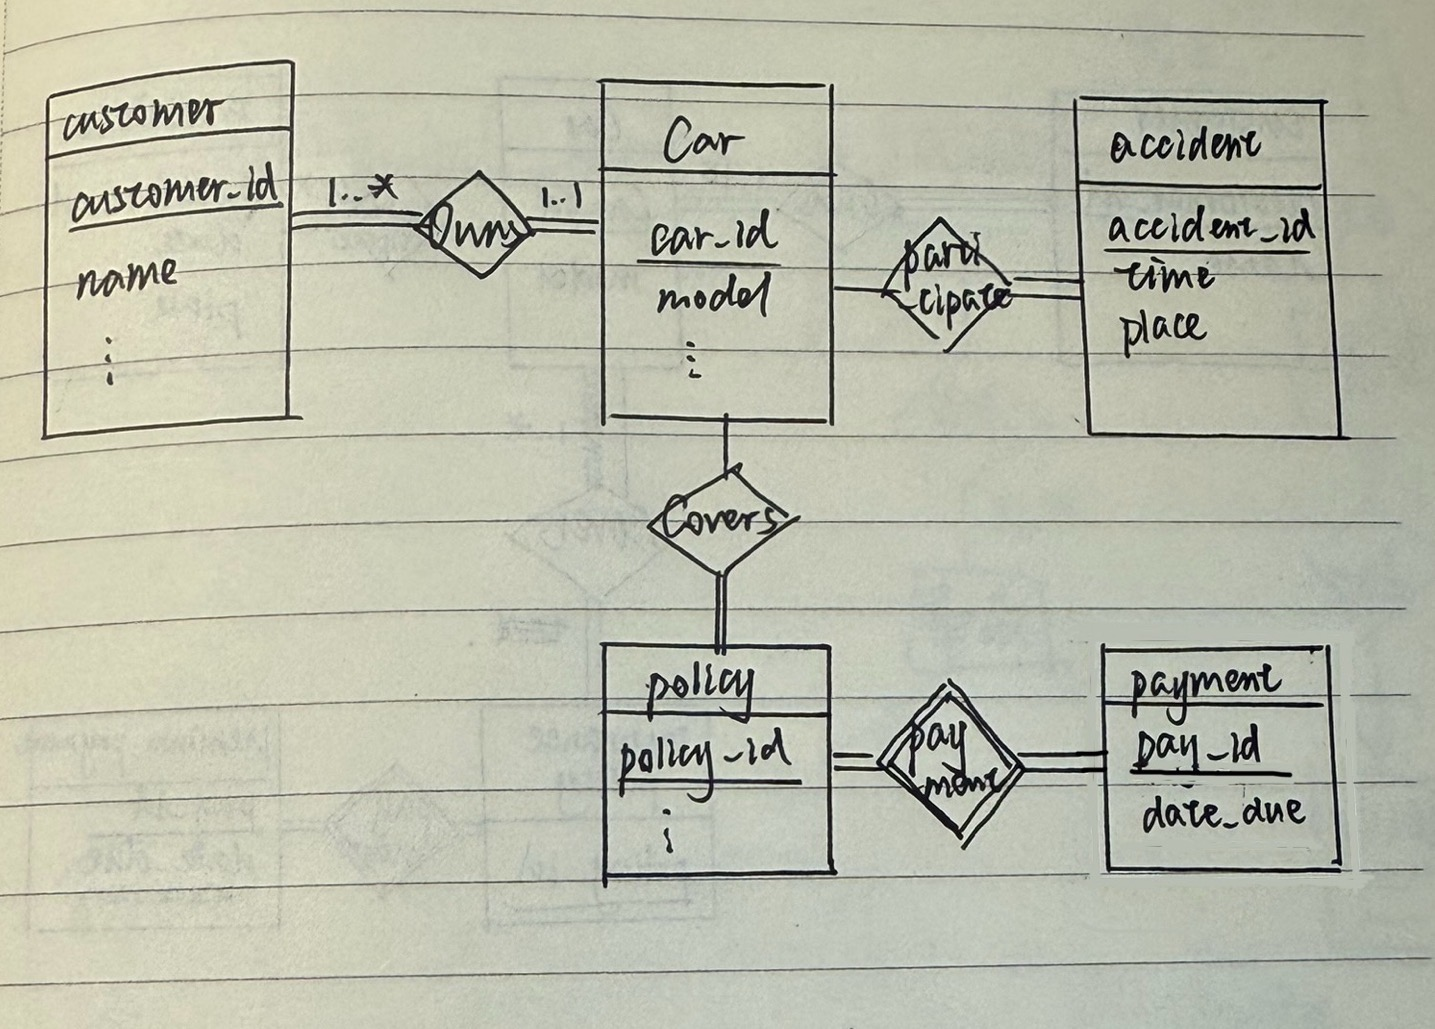
\includegraphics[width=10cm]{./images/6.1.jpg}
		\caption{6.1 解答}
	\end{figure}
	
	\section*{6.3}
	
	Design an E-R diagram for keeping track of the scoring statistics of your favorite sports team. You should store the matches played, the scores in each match, the players in each match, and individual player scoring statistics for each match.
	
	\section*{6.3 解答}
	
	\begin{figure}[H]
		\centering
		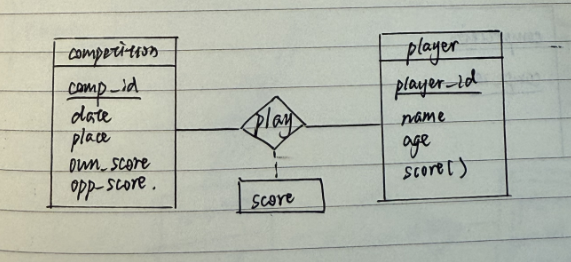
\includegraphics[width=11cm]{./images/6.3.png}
		\caption{6.3 解答}
	\end{figure}
	
	\section*{6.6}
	
	Consider the representation of the ternary relationship of Figure 6.29a using the binary relationships illustrated in Figure 6.29b (attributes not shown).
	
		\begin{enumerate}
			\item Show a simple instance of $ E $, $ A $, $ B $, $ C $, $ R_A $, $ R_B $, and $ R_C $ that cannot correspond to any instance of $ A $, $ B $, $ C $, and $ R $.
			\item Modify the E-R diagram of Figure 6.29b to introduce constraints that will guarantee that any instance of $ E $, $ A $, $ B $, $ C $, $ R_A $, $ R_B $, and $ R_C $ that satisfies the constraints will correspond to an instance of $ A $, $ B $, $ C $, and $ R $.
			\item Modify the preceding translation to handle total participation constraints on the ternary relationship.
		\end{enumerate}
	
	\begin{figure}[H]
		\centering
		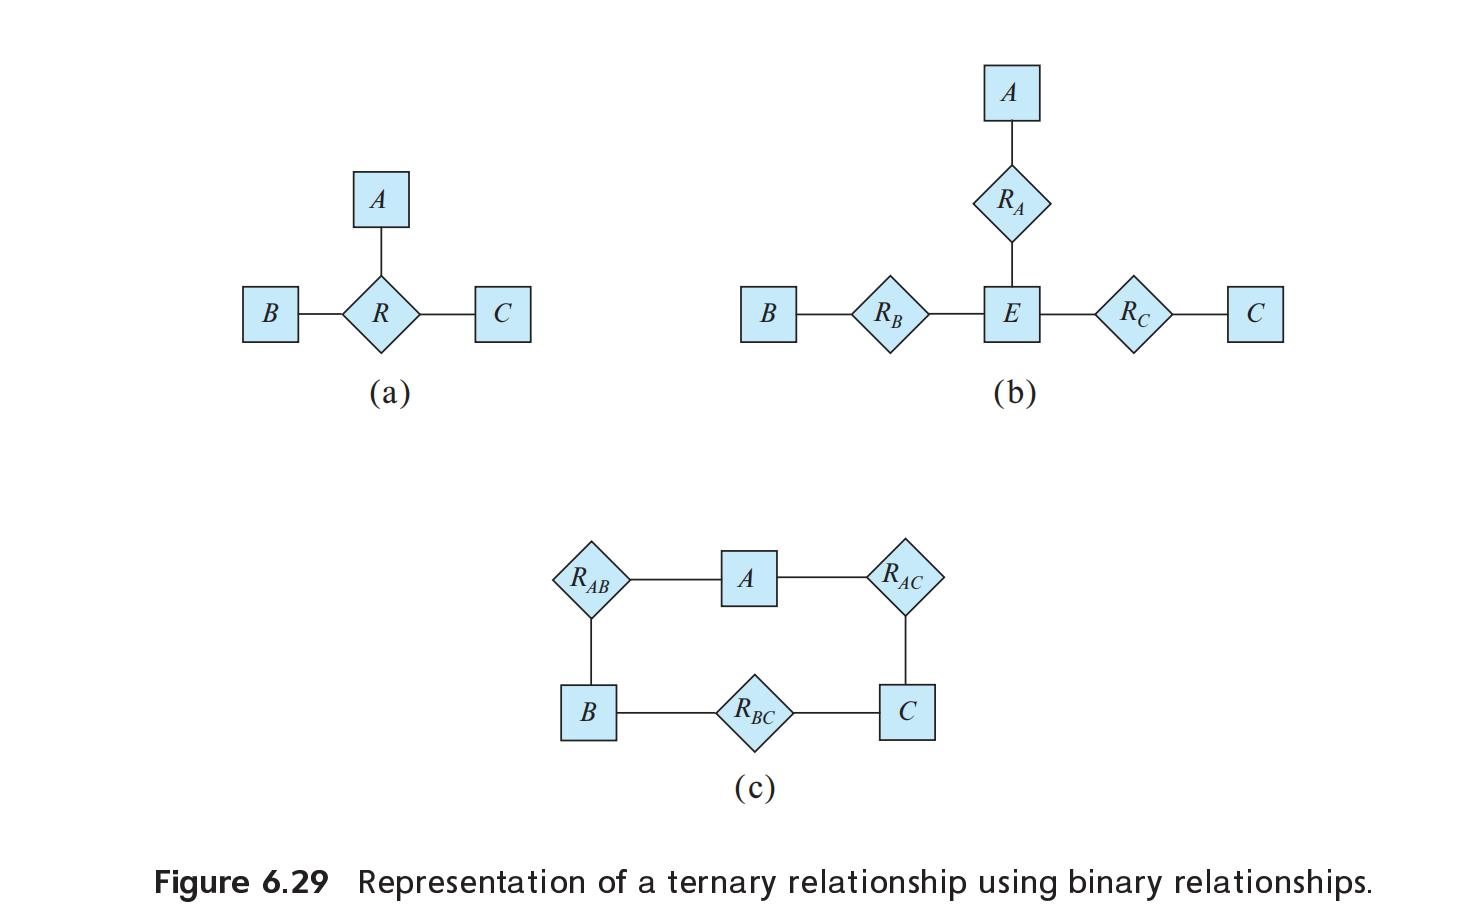
\includegraphics[width=9cm]{./images/homework 6.jpg}
		\caption{Figure 6.29}
	\end{figure}
	
	\section*{6.6 解答}
	
	\begin{enumerate}[noitemsep, label={{\arabic*})}]
		\item 假设 $ E = \{e_1, e_2\} $,$ A = \{a_1, a_2\} $,$ B = \{b_1\} $,$ C = \{c_1\} $,$ R_A = \{(e_1, a_1), (e_2, a_2)\} $,$ R_B = \{(e_1, b_1)\} $,$ R_C = \{(e_1, c_1)\} $。我们看到,由于元组 $ (e_2, a_2) $,不存在任何 $ A $,$ B $,$ C $ 和 $ R $ 的实例对应于 $ E $,$ R_A $,$ R_B $ 和 $ R_C $。
		
		\item 确保 $E$ 和 $R_A$, $R_B$, $R_C$ 之间都是完全参与的关系
		
		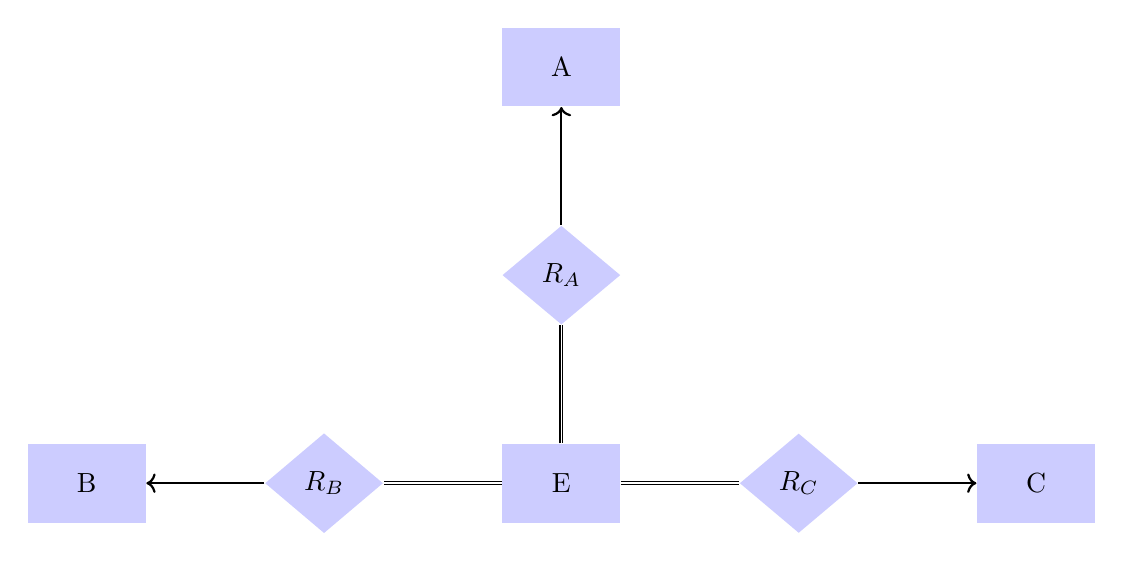
\begin{tikzpicture}[
			node distance=1.5cm,
			every node/.style={fill=blue!20},
			process/.style={rectangle, minimum width=1.5cm, minimum height=1cm, text centered},
			relation/.style={diamond, minimum width=1.5cm, minimum height=1cm, text centered},
			arrow/.style={rounded corners=4mm, draw, black, thick,-{Arrow[length=3mm,width=2mm]}}
			]
			
			% 节点定义
			\node (E) [process] {E};
			\node (RB) [relation, left=of E] {$R_B$};
			\node (B) [process, left=of RB] {B};
			\node (RC) [relation, right=of E] {$R_C$};
			\node (C) [process, right=of RC] {C};
			\node (RA) [relation, above=of E] {$R_A$};
			\node (A) [process, above=of RA] {A};
			
			% 边缘箭头
			\draw [=, double] (E) -- (RB);
			\draw [->, thick] (RB) -- (B);
			\draw [=, double] (E) -- (RA);
			\draw [->, thick] (RA) -- (A);
			\draw [=, double] (E) -- (RC);
			\draw [->, thick] (RC) -- (C);
			
		\end{tikzpicture}
		
		\item 确保 $R_A$, $R_B$, $R_C$ 和 $A$, $B$, $C$ 之间都是完全参与的关系
		
		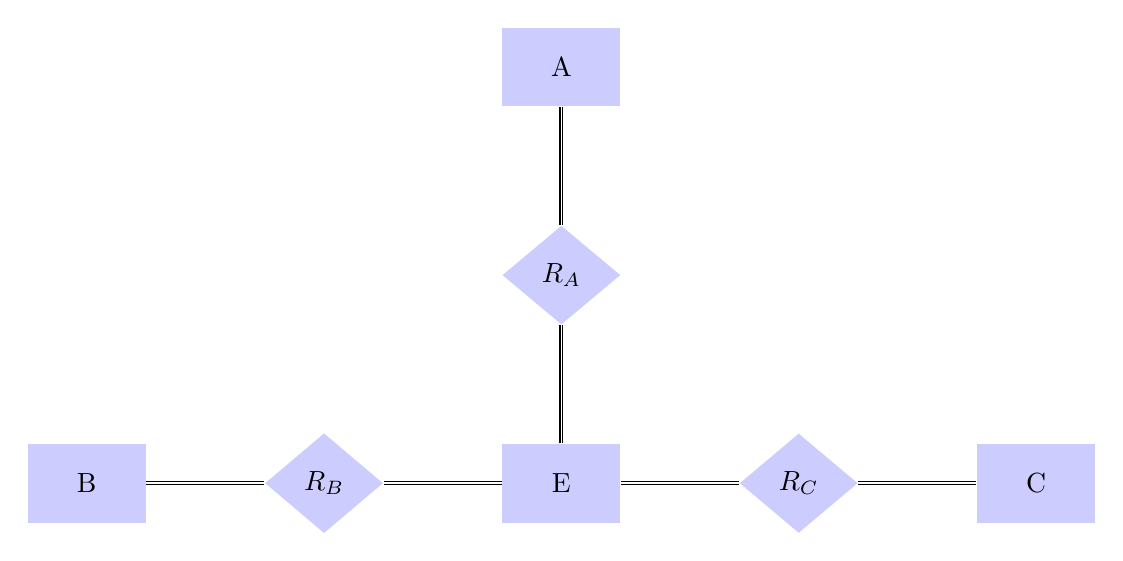
\begin{tikzpicture}[
			node distance=1.5cm,
			every node/.style={fill=blue!20},
			process/.style={rectangle, minimum width=1.5cm, minimum height=1cm, text centered},
			relation/.style={diamond, minimum width=1.5cm, minimum height=1cm, text centered},
			arrow/.style={rounded corners=4mm, draw, black, thick,-{Arrow[length=3mm,width=2mm]}}
			]
			
			% 节点定义
			\node (E) [process] {E};
			\node (RB) [relation, left=of E] {$R_B$};
			\node (B) [process, left=of RB] {B};
			\node (RC) [relation, right=of E] {$R_C$};
			\node (C) [process, right=of RC] {C};
			\node (RA) [relation, above=of E] {$R_A$};
			\node (A) [process, above=of RA] {A};
			
			% 边缘箭头
			\draw [=, double] (E) -- (RB);
			\draw [=, double] (RB) -- (B);
			\draw [=, double] (E) -- (RA);
			\draw [=, double] (RA) -- (A);
			\draw [=, double] (E) -- (RC);
			\draw [=, double] (RC) -- (C);
			
		\end{tikzpicture}
	\end{enumerate}\textbf{}
	
\end{document}
